% !TeX program = xelatex
\documentclass[10pt]{beamer}

\usetheme{metropolis}

\usepackage{pgfplots}
\usepgfplotslibrary{fillbetween}
\usepackage{pgfopts}
\usepackage{amsmath}
\usepackage{structuralanalysis}
\usepackage{tikz}
\usepackage{tikz-3dplot}
\usepackage{chngcntr}
\usepackage{wasysym}
\usepackage{mathtools}
\usepackage{alphalph}
\usepackage{xcolor}
\usepackage[showdow=false, en-US]{datetime2}

\newcommand{\highlight}[1]{%
	\colorbox{red!50}{$\displaystyle#1$}}

\setcounter{lecture}{6}
\counterwithin{equation}{lecture}
\makeatletter
\def\user@resume{resume}
\def\user@intermezzo{intermezzo}
%
\newcounter{previousequation}
\newcounter{lastsubequation}
\newcounter{savedparentequation}
\setcounter{savedparentequation}{1}
% 
\renewenvironment{subequations}[1][]{%
	\def\user@decides{#1}%
	\setcounter{previousequation}{\value{equation}}%
	\ifx\user@decides\user@resume 
	\setcounter{equation}{\value{savedparentequation}}%
	\else  
	\ifx\user@decides\user@intermezzo
	\refstepcounter{equation}%
	\else
	\setcounter{lastsubequation}{0}%
	\refstepcounter{equation}%
	\fi\fi
	\protected@edef\theHparentequation{%
		\@ifundefined {theHequation}\theequation \theHequation}%
	\protected@edef\theparentequation{\theequation}%
	\setcounter{parentequation}{\value{equation}}%
	\ifx\user@decides\user@resume 
	\setcounter{equation}{\value{lastsubequation}}%
	\else
	\setcounter{equation}{0}%
	\fi
	\def\theequation  {\theparentequation  \alph{equation}}%
	\def\theHequation {\theHparentequation \alph{equation}}%
	\ignorespaces
}{%
%  \arabic{equation};\arabic{savedparentequation};\arabic{lastsubequation}
\ifx\user@decides\user@resume
\setcounter{lastsubequation}{\value{equation}}%
\setcounter{equation}{\value{previousequation}}%
\else
\ifx\user@decides\user@intermezzo
\setcounter{equation}{\value{parentequation}}%
\else
\setcounter{lastsubequation}{\value{equation}}%
\setcounter{savedparentequation}{\value{parentequation}}%
\setcounter{equation}{\value{parentequation}}%
\fi\fi
%  \arabic{equation};\arabic{savedparentequation};\arabic{lastsubequation}
\ignorespacesafterend
}
\makeatother
\title{AE 737 - Mechanics of Damage Tolerance}
\subtitle{Lecture \arabic{lecture}}
\date{Last Updated: \today\ at \DTMcurrenttime}
\author{Dr. Nicholas Smith}
\institute{Wichita State University, Department of Aerospace Engineering}
% \titlegraphic{\hfill\includegraphics[height=1.5cm]{logo/logo}}

\begin{document}

\maketitle
\begin{frame}{schedule}
	\begin{itemize}
		\item 9 Feb - Fracture Toughness, Homework 2 Due, Homework 3 Assigned
		\item 11 Feb - Fracture Toughness
		\item 16 Feb - Residual Strength, Homework 3 Due, Homework 4 Assigned
		\item 18 Feb - Residual Strength
		\item 23 Feb - Multiple Site Damage, Homework 4 Due, Homework 5 Assigned
		\item 25 Feb - Mixed-mode Fracture
	\end{itemize}
\end{frame}

\begin{frame}
  \frametitle{outline}
  \setbeamertemplate{section in toc}[sections numbered]
  \tableofcontents[hideallsubsections]
\end{frame}

\section{fracture toughness}

\begin{frame}{fracture toughness}
	\begin{itemize}
		\item The critical load at which a cracked specimen fails produces a critical stress intensity factor
		\item The "critical stress intensity factor" is known as $K_c$
		\item For Mode I, this is called $K_{Ic}$
		\item The critical stress intensity factor is also known as fracture toughness
		\begin{equation}
		K_{IC} = \sigma_c \sqrt{\pi a}\beta
		\end{equation}
		\pause
		\item NOTE: "Fracture Toughness" can also refer to $G_{Ic}$, which is analogous to $K_{Ic}$, but not the same
	\end{itemize}
\end{frame}

\begin{frame}{fracture toughness}
	\begin{itemize}
		\item Fracture toughness is a material property, but it is only well-defined in certain conditions
		\item Brittle materials
		\item Plane strain (smaller plastic zone)
		\item In these cases ASTM E399-12 is used.
	\end{itemize}
\end{frame}

\begin{frame}{fracture toughness}
	\begin{figure}
	\centering
	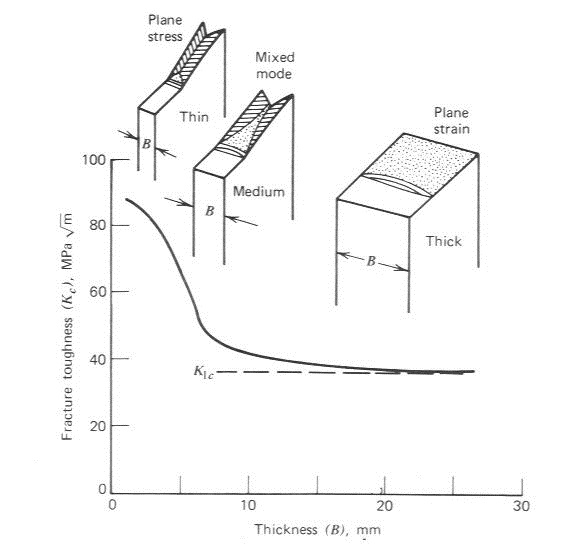
\includegraphics[width=0.7\linewidth]{KIC_thickness}
	\label{fig:KIC_thickness}
\end{figure}
\end{frame}

\begin{frame}{fracture toughness}
	\begin{itemize}[<+->]
		\item "Stable" vs. "unstable" crack growth
		\item Stable crack growth means the crack extends only with increased load
		\item Unstable crack growth means the crack will continue to extend indefinitely under the same load
		\item For a perfectly brittle material, there is no stable crack growth, as soon as a critical load is reached, the crack will extend indefinitely
		\item For an elastic-plastic material, once the load is large enough to extend the crack, it will extend slightly
		\item The load must be continually increased until a critical value causes unstable crack growth
	\end{itemize}
\end{frame}

\begin{frame}{fracture toughness}
	\begin{itemize}[<+->]
		\item During an experiment, we will record the crack length and applied load ($P_i$, $a_i$) each time we increase the load
		\item We can calculate a unique stress intensity factor $K_{Ii}$ at each of these points
		\item These are then used to create a "K-curve", plotting $K_I$ vs. $a$
	\end{itemize}
\end{frame}

\begin{frame}{K-curve}
	\begin{figure}
		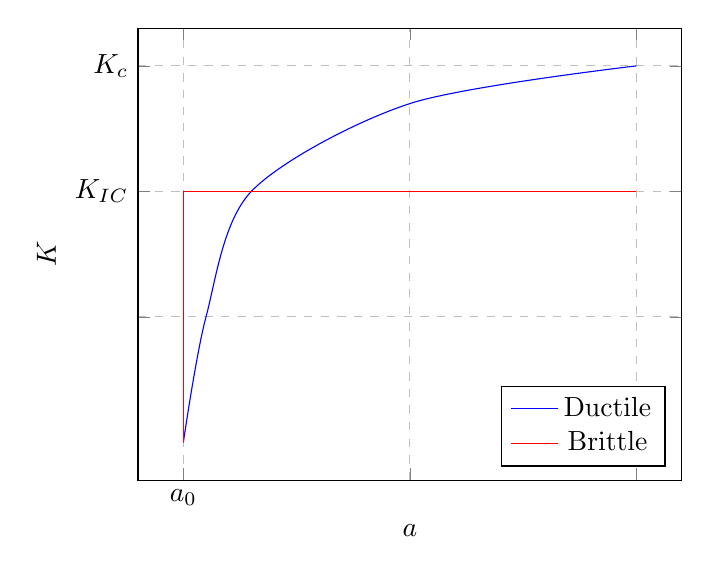
\begin{tikzpicture}
		\begin{axis}[
		width=0.7\linewidth,
		grid=major,
		grid style=dashed,
		xlabel=$a$,
		ylabel=$K$,
		xtick={1,2,3},
		xticklabels={$a_0$, , },
		ytick={0.5,1,1.5},
		yticklabels={ ,$K_{IC}$,$K_c$},
		legend entries={Ductile, Brittle},
		legend pos=south east,
		no markers
		]
		\addplot+[smooth]
		coordinates
		{(1,0) (1.1,0.5) (1.3,1) (2,1.35) (3,1.5)};
		\addplot+[const plot]
		coordinates
		{(1,0) (1,1) (3,1)};
		\end{axis}
		\end{tikzpicture}
	\end{figure}
\end{frame}

\begin{frame}{K-curve}
	\begin{itemize}[<+->]
		\item Materials will generally not be as flat as the perfectly brittle example
		\item Plane strain conditions and brittle materials will tend towards a "flat" K-curve
		\item $K_{IC}$ for brittle/plane strain is very well defined
		\item $K_C$ for plane stress can refer to two things
		\item Either the maximum $K_C$ during a test, or tangent point on $K_R$-curve (R-curve)
	\end{itemize}
\end{frame}

\begin{frame}{example - stable crack growth}
	\begin{itemize}[<+->]
		\item In composites, and adhesives, some  work is needed to ensure stable crack growth
		\item The Double-Cantilever Beam (DCB) experiment to find $G_{IC}$ illustrates this
		\begin{subequations}
			\begin{align}
			\label{eq:compliance}
			C &= \frac{\delta}{P}\\
			C &= \frac{2a^3}{3EI}\\
			G &= \frac{P^2}{2b}\frac{dC}{da}\\
			G &= \frac{P^2a^2}{bEI}
			\end{align}
		\end{subequations}
		\item For crack growth to be stable we need
		\begin{equation}
		\frac{dG}{da} \le 0
		\end{equation}
	\end{itemize}
\end{frame}

\begin{frame}{example - stable crack growth}
	\begin{itemize}[<+->]
		\item Under fixed-load conditions, we find
		\begin{equation}
		\frac{dG}{da} = \frac{2P^2a}{bEI}
		\end{equation}
		\item This is always positive, and thus results in unstable crack growth
		\item Under fixed-displacement conditions, we substitute for $P$ using (\ref{eq:compliance})
		\item We find
		\begin{equation}
		\frac{dG}{da} = -\frac{9\delta^2EI}{ba^3}
		\end{equation}
		\item Which is always stable, so for DCB tests, displacement control is generally used
	\end{itemize}
\end{frame}

\section{plane strain, brittle}

\begin{frame}{plane strain, brittle}
\begin{itemize}
	\item For relatively brittle materials, we don't need to worry about the R-curve
	\item Specimens are made according to these specifications
	\begin{subequations}
		\label{eq:specimen}
		\begin{align}
		a \ge 2.5 \left(\frac{K_{IC}}{\sigma_{YS}}\right)^2\\
		b \ge 2.5 \left(\frac{K_{IC}}{\sigma_{YS}}\right)^2\\
		W \ge 5 \left(\frac{K_{IC}}{\sigma_{YS}}\right)^2
		\end{align}
	\end{subequations}
\end{itemize}
\end{frame}

\begin{frame}{ASTM E399}
	\begin{enumerate}
		\item Select specimen size (see (\ref{eq:specimen}))
		\item Select specimen type (Compact Tension or Single Edge Notched Bend)
	\end{enumerate}
\end{frame}

\begin{frame}{ASTM E399}
	\begin{figure}
	\centering
	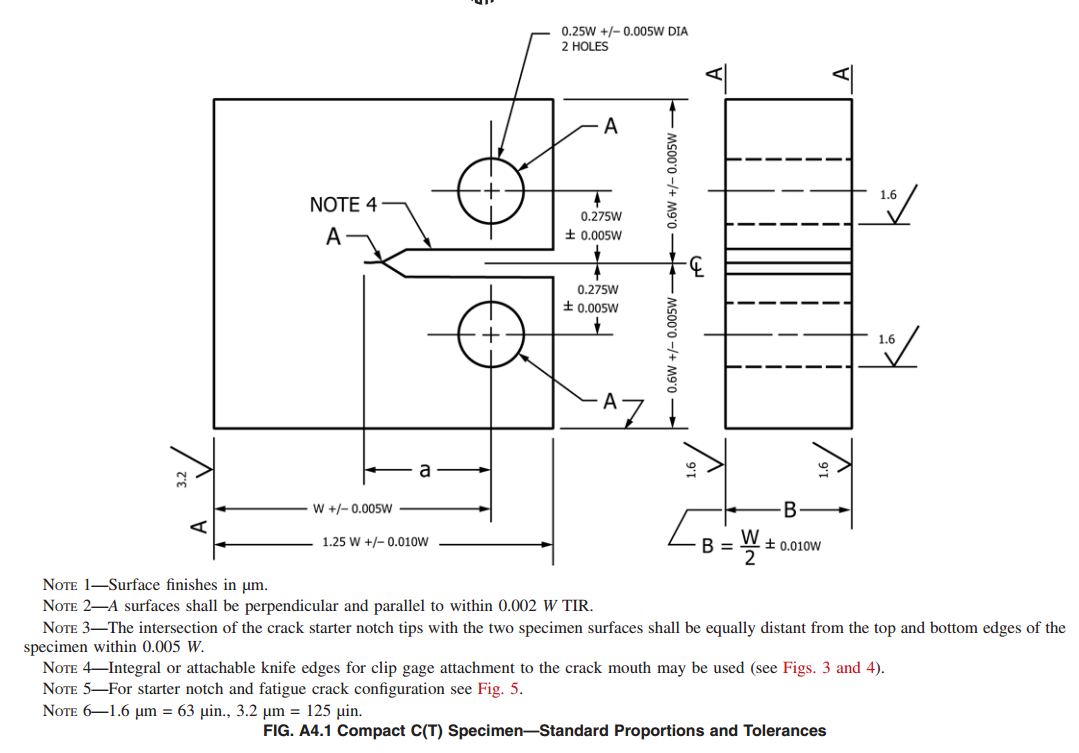
\includegraphics[width=0.7\linewidth]{CT}
	\label{fig:CT}
	\end{figure}
\end{frame}

\begin{frame}{ASTM E399}
	\begin{figure}
	\centering
	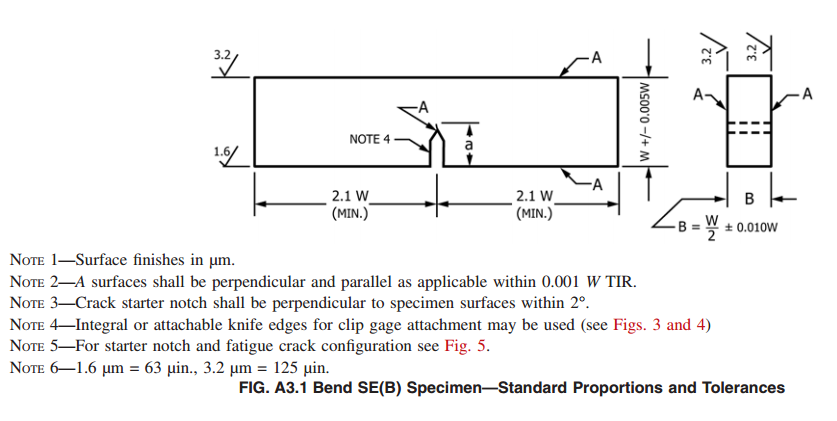
\includegraphics[width=0.7\linewidth]{SENB}
	\label{fig:SENB}
	\end{figure}
\end{frame}

\begin{frame}{ASTM E399}
	\begin{figure}
	\centering
	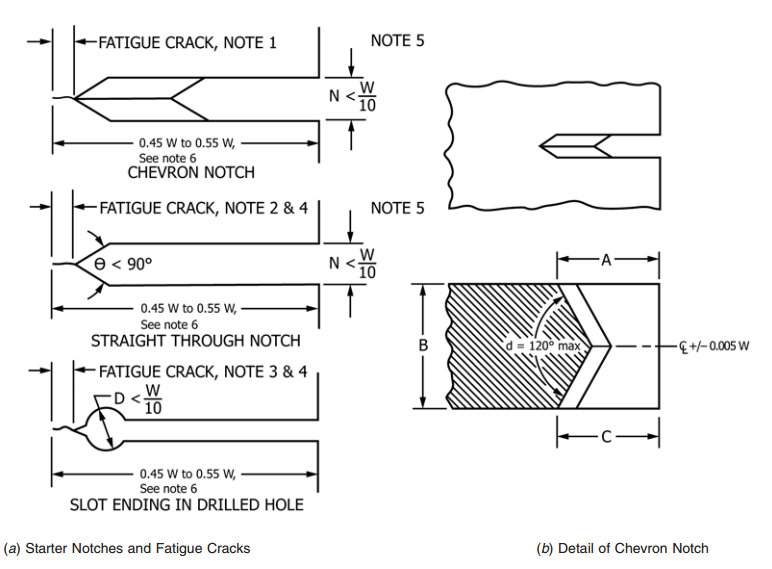
\includegraphics[width=0.7\linewidth]{chevron}
	\label{fig:chevron}
	\end{figure}
\end{frame}

\begin{frame}{ASTM E399}
	\begin{enumerate}\setcounter{enumi}{2}
		\item Machine specimen
		\item Fatigue crack specimen $K_f < 0.6 K_{IC}$
		\begin{itemize}
			\item This is to ensure that the plastic zone size during fatigue is smaller than the plastic zone size during testing
			\item If $K_{IC}$ has not yet been determined, you may have to guess the first time
		\end{itemize}
	\end{enumerate}
\end{frame}

\begin{frame}{ASTM E399}
	\begin{enumerate}\setcounter{enumi}{4}
		\item Mount specimen, attach gage
		\item Load rate should ensure "static" load conditions. (30 - 150 ksi$\sqrt{\text{in.}}$/min.)
		\item Determine the "provisional" value of $K_{IC}$ (known as $K_Q$)
		\begin{figure}
			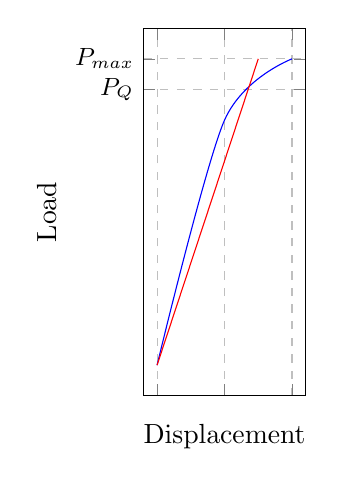
\begin{tikzpicture}
			\begin{axis}[
			width=0.3\linewidth,
			grid=major,
			grid style=dashed,
			xlabel=Displacement,
			ylabel=Load,
			xtick={},
			xticklabels={},
			ytick={4.5,5},
			yticklabels={\small $P_{Q}$,\small $P_{max}$},
			y post scale = 3,
			no markers
			]
			\addplot+[smooth]
			coordinates
			{(0,0) (1,4) (2,5)};
			\addplot+
			coordinates
			{(0,0) (1.5,5)};
			\end{axis}
			\end{tikzpicture}
			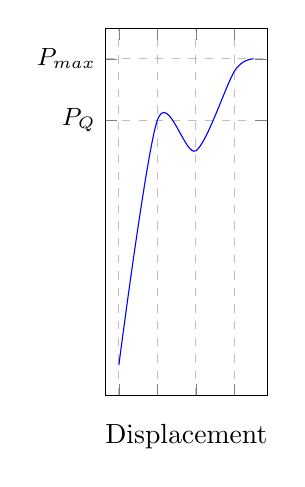
\begin{tikzpicture}
			\begin{axis}[
			width=0.3\linewidth,
			grid=major,
			grid style=dashed,
			xlabel= Displacement,
			xtick={},
			xticklabels={},
			ytick={4,5},
			yticklabels={\small $P_{Q}$,\small $P_{max}$},
			y post scale = 3,
			no markers
			]
			\addplot+[smooth]
			coordinates
			{(0,0) (1,4) (2,3.5) (3,4.8) (3.5,5)};
			\end{axis}
			\end{tikzpicture}
			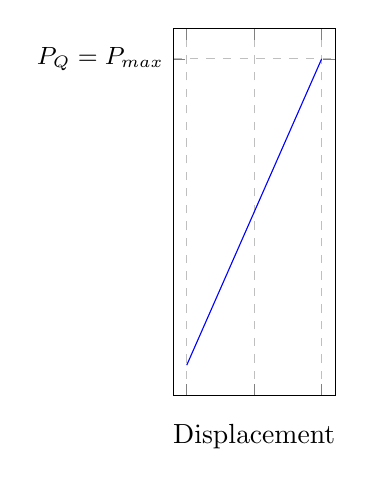
\begin{tikzpicture}
			\begin{axis}[
			width=0.3\linewidth,
			grid=major,
			grid style=dashed,
			xlabel= Displacement,
			xtick={},
			xticklabels={},
			ytick={4},
			yticklabels={\small $P_{Q}=P_{max}$},
			y post scale = 3,
			no markers
			]
			\addplot+[smooth]
			coordinates
			{(0,0) (1,4)};
			\end{axis}
			\end{tikzpicture}
		\end{figure}
	\end{enumerate}
\end{frame}

\begin{frame}{ASTM E399}
	\begin{enumerate} \setcounter{enumi}{7}
		\item[]
		\begin{enumerate}[<+->]
			\item If the load-displacement curve is like the first figure, with some non-linearity, we let $P_Q$ be the point of intersection between the load-displacement curve and a line whose slope is 5\% lower than the slope in the elastic region
			\item "Pop-in" occurs when there is stable crack extension before the plasticity begins. We let $P_Q$ bet the point where stable crack extension begins.
			\item For a perfectly linear material, $P_Q = P_{max}$.
			\item[]
			\begin{align}
			K_Q &= \frac{P_Q}{BW^{1/2}}f\left(\frac{a}{W}\right) & \text{Compact Tension}\\
			K_Q &= \frac{P_Q}{BW^{3/2}}g\left(\frac{a}{W}\right) & \text{SENB}
			\end{align}
		\end{enumerate}
		
	\end{enumerate}
\end{frame}

\begin{frame}{ASTM E399}
	\begin{enumerate}[<+->]\setcounter{enumi}{7}
		\item Ensure that your specimen is still valid
		\begin{align}
		a \ge 2.5 \left(\frac{K_Q}{\sigma_{YS}}\right)^2\\
		b \ge 2.5 \left(\frac{K_Q}{\sigma_{YS}}\right)^2\\
		W \ge 5 \left(\frac{K_Q}{\sigma_{YS}}\right)^2
		\end{align}
		\begin{itemize}[<+->]
		\item For stable crack extension, check the $P_{max}$
		\begin{equation}
		\frac{P_{max}}{P_Q} \le 1.10
		\end{equation}
		\item Check for symmetric crack front, $a_1$, $a_2$, and $a_3$ must be within 5\% of $a$. $a_s$ must be within 10\% of $a$.
		\begin{equation}
		\frac{a_1 + a_2 + a_3}{3} = a
		\end{equation}
		\item Load-displacement should have an initial slope between 0.7 and 1.5
		\end{itemize}
	\end{enumerate}
\end{frame}

\section{plane stress, ductile}

\begin{frame}{R-curve}
	\begin{itemize}[<+->]
		\item For materials with some plasticity, the $K_R$ Curve, or R Curve, is very important
		\item Sometimes called a "resistance curve" it is generally dependent on
		\begin{itemize}[<+->]
			\item Thickness
			\item Temperature
			\item Strain rate
		\end{itemize}
		\item When done correctly, $K_R$ curves are not dependent on initial crack size or the specimen type used
		\item ASTM E561
	\end{itemize}
\end{frame}

\begin{frame}{ASTM E561}
	\begin{itemize}[<+->]
		\item Compact Tension (CT or C(T)) specimens may be used for plane stress $K_R$ curves
		\item The other specimen which is permitted is a middle-cracked tension specimen (M(T))
		\item M(T) specimens are preferred in many cases due to a more uniform stress distribution (particularly important for anisotropic materials)
	\end{itemize}
\end{frame}

\begin{frame}{ASTM E561}
	
\begin{figure}
\centering
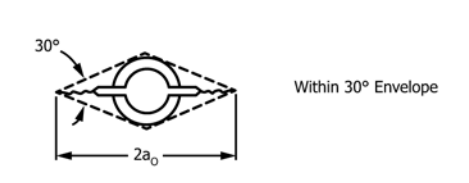
\includegraphics[width=0.5\linewidth]{MT-envelope}
\label{fig:MT-envelope}
\end{figure}
\begin{figure}
\centering
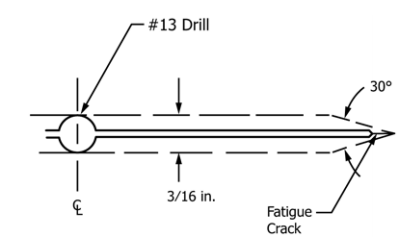
\includegraphics[width=0.6\linewidth]{MT-notch}
\label{fig:MT-notch}
\end{figure}

\end{frame}

\begin{frame}{minimum sample dimensions}
	
\begin{figure}
\centering
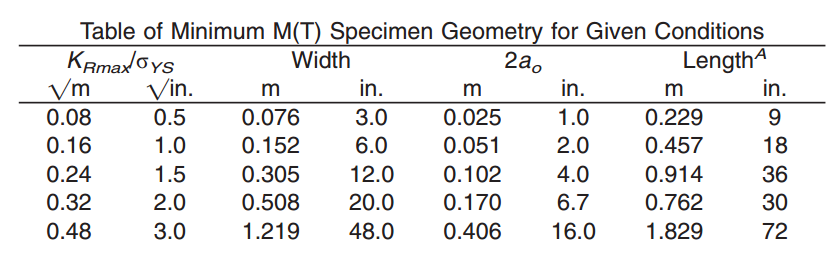
\includegraphics[width=0.6\linewidth]{MT-minimum}
\caption{M(T) minimum recommended dimensions}
\label{fig:MT-minimum}
\end{figure}

\begin{figure}
\centering
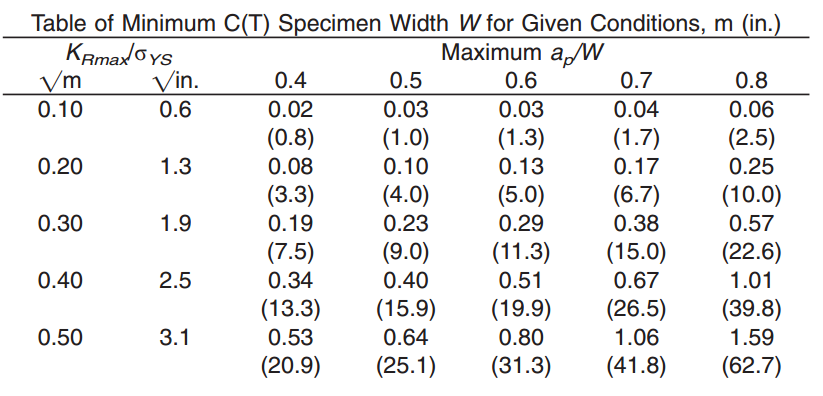
\includegraphics[width=0.6\linewidth]{CT-minimum}
\caption{C(T) minimum recommended dimensions}
\label{fig:CT-minimum}
\end{figure}

\end{frame}

\begin{frame}{effective crack length}
	\begin{itemize}
		\item ASTM E561 describes three ways to obtain the effective crack length during testing
		\begin{enumerate}[<+->]
			\item Measure the crack length visually and calculate $r_p$
			\item Measure crack length using "unloading compliance" and adding plastic zone size
			\item Measure the effective crack size directly using "secant compliance"
		\end{enumerate}
	\end{itemize}
\end{frame}

\begin{frame}{secant compliance}
	\begin{figure}
	\centering
	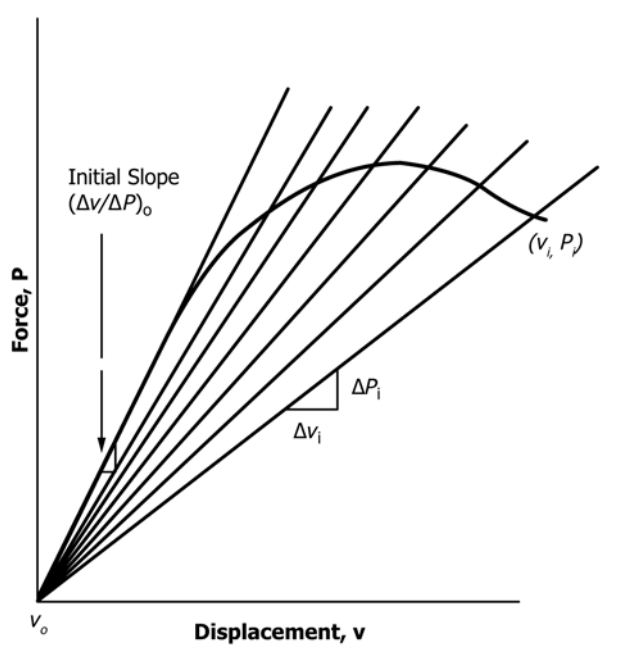
\includegraphics[width=0.7\linewidth]{secant}
	\label{fig:secant}
	\end{figure}
\end{frame}

\begin{frame}{secant compliance M(T)}
	\begin{itemize}[<+->]
		\item Using the slope data from our load-displacement curve, we can calculate the effective crack length using
		\begin{multline}
		EB\left(\frac{\Delta v}{\Delta P}\right) = \frac{2 Y}{W} \sqrt{\frac{\pi a / W}{\sin (\pi a / W)}} \\
		\qquad \left[\frac{2W}{\pi Y} \cosh^{-1} \left(\frac{\cosh(\pi Y/W)}{\cos (\pi a / W)}\right) - \frac{1+\nu}{\sqrt{1 + \left(\frac{\sin(\pi a/W)}{\sinh (\pi Y/W)}\right)^2}}+\nu\right]
		\end{multline}
	\end{itemize}
\end{frame}

\begin{frame}{secant compliance M(T)}
	\begin{itemize}[<+->]
		\item This equation is difficult to solve directly for $a$ (for M(T) specimens) 
		\item Instead it is generally solved iteratively
		\item The following equations are used to give a good initial guess to use in iterations
		\begin{align}
		X &= 1 - \exp \left[\frac{-\sqrt{[EB(\Delta v/ \Delta P)]^2 - (2Y/W)^2}}{2.141}\right]\\
		&\begin{aligned}
		\mathllap{\frac{2a}{W}} &= 1.2235X - 0.699032X^2 + 3.25584X^3 - 6.65042X^4 + \\
		&\qquad5.54X^5 - 1.66989X^6
		\end{aligned}
		\end{align}
	\end{itemize}
\end{frame}

\begin{frame}{secant compliance M(T)}
	\begin{itemize}
		\item In the above equations, the following are the definitions of parameters used
		\begin{align*}
		E &= \qquad \text{Young's Modulus}\\
		\Delta v / \Delta P &= \qquad \text{specimen compliance}\\
		B &= \qquad \text{specimen thickness}\\
		W &= \qquad \text{specimen width}\\
		Y &= \qquad \text{half span of the displacement measurement points}\\
		a &= \qquad \text{effective crack length}\\
		\nu &= \qquad \text{Poisson's ratio}
		\end{align*}
	\end{itemize}
\end{frame}

\begin{frame}{secant compliance C(T)}
	\begin{itemize}[<+->]
		\item For C(T) specimens, we use the following equations
		\item[]
		\begin{equation}
		EB\frac{\Delta v}{\Delta P} = A_0 + A_1\left(\frac{a}{W}\right) + A_2\left(\frac{a}{W}\right)^2 + A_3\left(\frac{a}{W}\right)^3 + A_4\left(\frac{a}{W}\right)^4
		\end{equation}
		\item The coefficients will differ based on where the displacement is measured from
	\end{itemize}
\end{frame}

\begin{frame}{secant compliance C(T)}
\begin{figure}
\centering
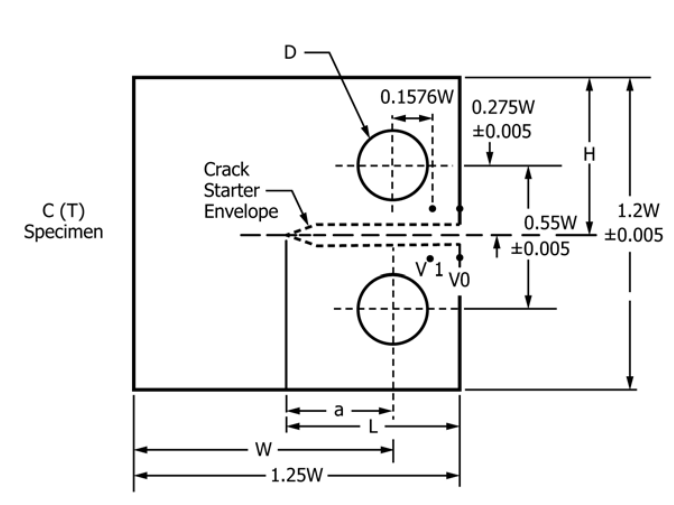
\includegraphics[width=0.7\linewidth]{CT-KR}
\label{fig:CT-KR}
\end{figure}
\end{frame}

\begin{frame}{secant compliance C(T)}
	\begin{tabular}{rrrrrr}
	location	& $A_0$ & $A_1$ & $A_2$ & $A_3$ & $A_4$ \\ 
	\hline
	$V_0$	& 120.7 & -1065.3 & 4098.0 & -6688.0 & 4450.5 \\ 
	$V_1$	& 103.8 & -930.4 & 3610.0 & -5930.5 & 3979.0
	\end{tabular} 
	\begin{tabular}{rrrrrrr}
		location	& $C_0$ & $C_1$ & $C_2$ & $C_3$ & $C_4$ & $C_5$ \\ 
		\hline
		$V_0$	& 1.0010 & -4.6695 & 18.460 & -236.82 & 1214.90 & -2143.6\\ 
		$V_1$	& 1.0008 & -4.4473 & 15.400 & -180.55 & 870.92 & -1411.3
	\end{tabular} 
\end{frame}

\begin{frame}{secant compliance C(T)}
	\begin{itemize}
		\item Where the initial guess for $a$ is provided by
		\begin{equation}
		\frac{a}{W} = C_0 + C_1 U + C_2 U^2 + C_3 U^3 + C_4 U^4 + C_5 U^5
		\end{equation}
		\item and $U$ is given by
		\begin{equation}
		U = \frac{1}{1 + \sqrt{EB\frac{\Delta v}{\Delta P}}}
		\end{equation}
	\end{itemize}
\end{frame}

\begin{frame}{buckling}
	\begin{itemize}
		\item If the test is stopped and re-started frequently (to measure crack length by hand or to use the compliance method of crack measurement) buckling can interfere with results
		
\begin{figure}
\centering
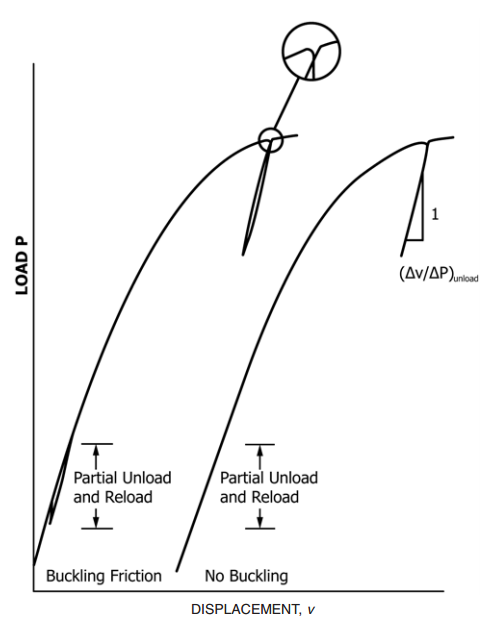
\includegraphics[width=0.5\linewidth]{buckling}
\label{fig:buckling}
\end{figure}
	\end{itemize}
\end{frame}

\begin{frame}{buckling}
	\begin{itemize}
		\item If buckling is shown to be present in the test, supports can be used to prevent buckling
		\item These supports can introduce friction
		\item They should be well-lubricated for accurate test results
	\end{itemize}
\end{frame}

\begin{frame}{net section stress}
	\begin{itemize}
		\item One final consideration when dealing with plane stress fracture mechanics is the net section stress
		\item For the test to be valid, failure must occur due to fracture, not general static failure
		\item Static failure will occur when $\sigma_{N} = \sigma_{YS}$
	\end{itemize}
\end{frame}

\begin{frame}{generate $K_R$ curve}
	\begin{itemize}[<+->]
		\item Once the effective crack length and $K_{Ie}$ has been determined for the test, we can generate the $K_R$ curve
		\item The $K_R$ curve is quite simply a plot of $K_{Ie}$ vs. $a$ for the test performed (i.e. with varying stress and increasing crack length)
		\item When the test is performed correctly, the $K_R$ curve is not a function of the initial crack length
		\item For this reason, we often plot $K_{Ie}$ vs. $\Delta a$, to subtract the initial crack length
		\item We can superpose constant-stress $K$-curves on this graph, the curve which intersects at a tangent point creates the most "standard" definition for $K_C$
	\end{itemize}
\end{frame}

\begin{frame}{example}
	
\begin{figure}
\centering
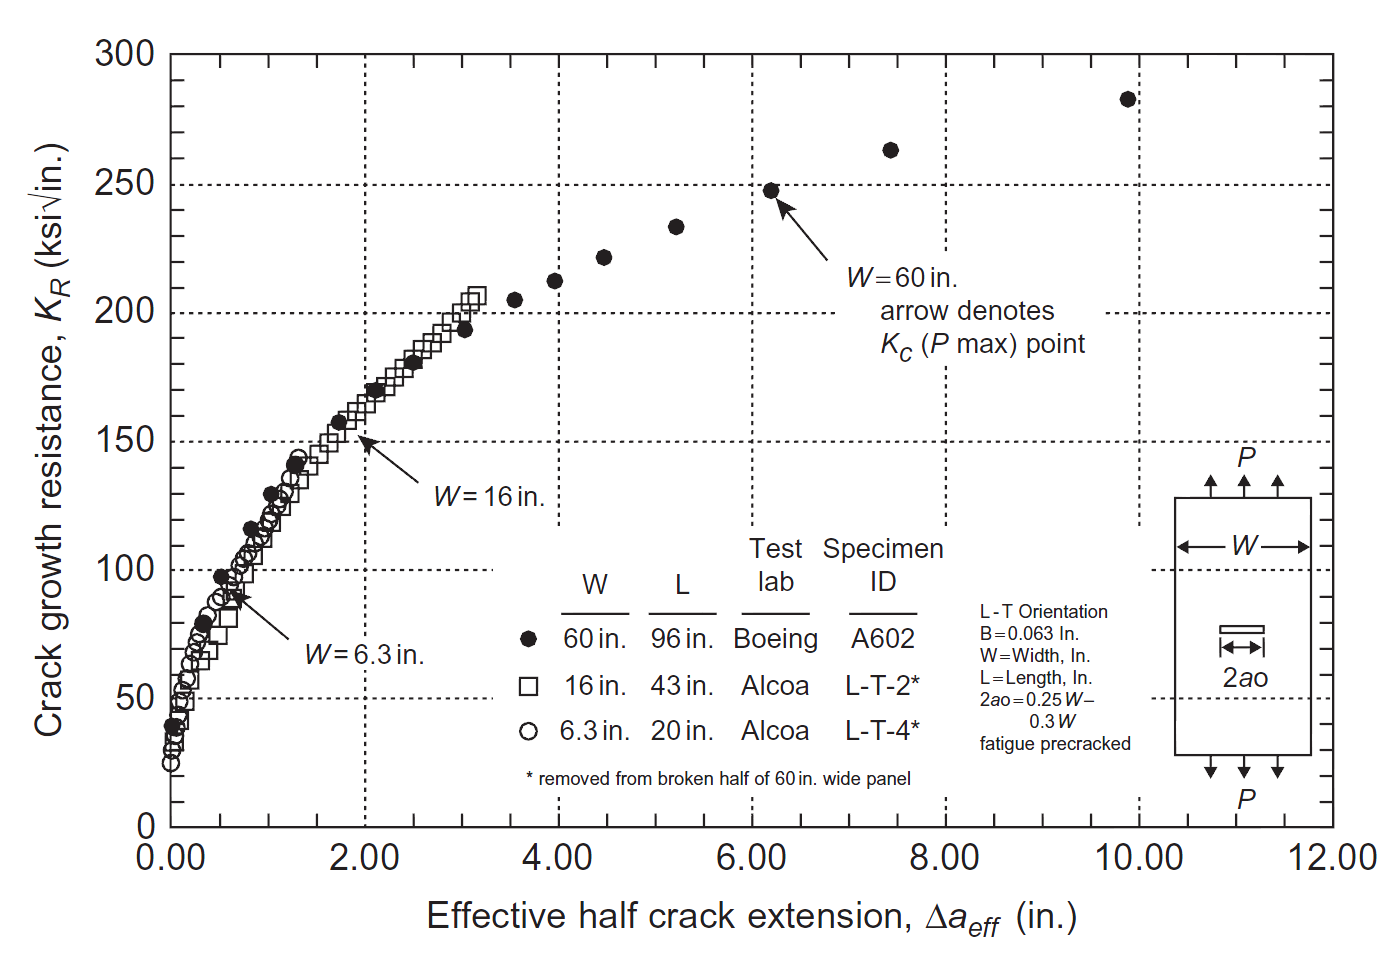
\includegraphics[width=0.7\linewidth]{KR_C188T3_aluminum}
\caption{$K_R$ Curve for C188-T3 aluminum for varying sample thickness (Boeing and Alcoa)}
\label{fig:KR_C188T3_aluminum}
\end{figure}
\end{frame}

\begin{frame}{example}
\begin{figure}
\centering
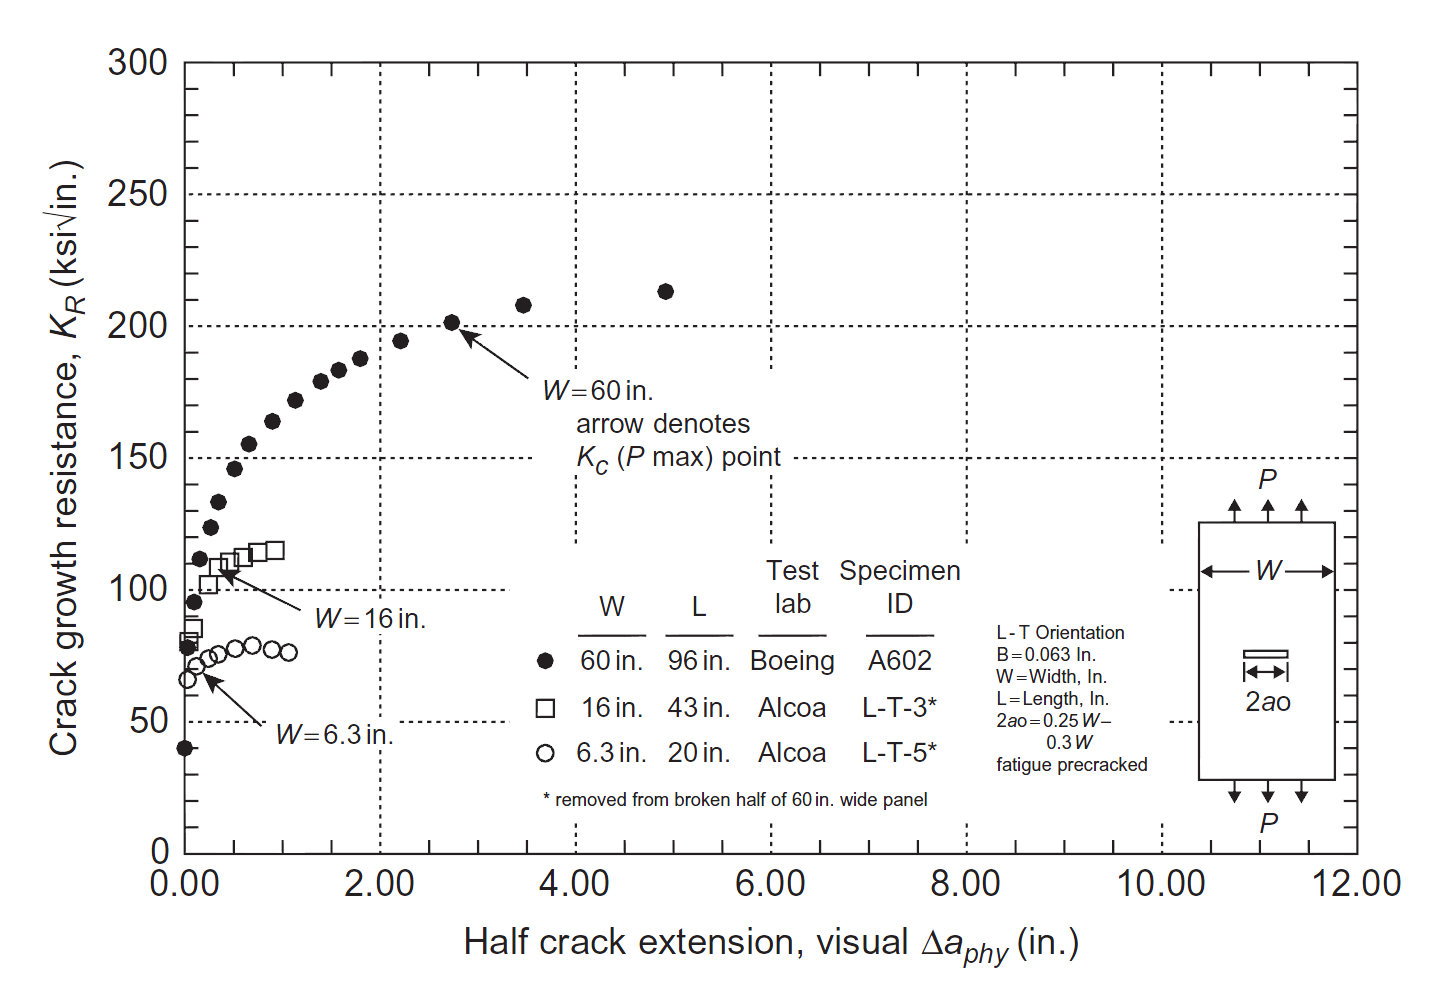
\includegraphics[width=0.7\linewidth]{KR_C188T3_physical}
\caption{$K_R$ curve for the same specimens, but without adjusting for the plastic zone size.}
\label{fig:KR_C188T3_physical}
\end{figure}
\end{frame}

\end{document}
